% THIS IS AN EXAMPLE DOCUMENT FOR VLDB 2012
% based on ACM SIGPROC-SP.TEX VERSION 2.7
% Modified by  Gerald Weber <gerald@cs.auckland.ac.nz>
% Removed the requirement to include *bbl file in here. (AhmetSacan, Sep2012)
% Fixed the equation on page 3 to prevent line overflow. (AhmetSacan, Sep2012)


\documentclass{vldb}
\usepackage{graphicx}
\usepackage{pgfplots}
\usepackage{balance}  % for  \balance command ON LAST PAGE  (only there!)
\usepackage{array}

% smart quotes
\usepackage [autostyle, english = american]{csquotes}
\MakeOuterQuote{"}

% Include information below and uncomment for camera ready
\vldbTitle{TLA+ Trace Checking In Production}
\vldbAuthors{A. Jesse Jiryu Davis, Judah Schvimer, Max Hirschhorn}
\vldbDOI{https://doi.org/10.14778/xxxxxxx.xxxxxxx}
\vldbVolume{12}
\vldbNumber{xxx}
\vldbYear{2019}

\begin{document}

% ****************** TITLE ****************************************

\title{TLA+ Trace Checking In Production}
% OUTLINE: https://docs.google.com/document/d/16qDw3hxpi64ASPm0j0HneQSjyY7Kf93tCCLzG1NdOFM/edit

% possible, but not really needed or used for PVLDB:
%\subtitle{[Extended Abstract]
%\titlenote{A full version of this paper is available as\textit{Author's Guide to Preparing ACM SIG Proceedings Using \LaTeX$2_\epsilon$\ and BibTeX} at \texttt{www.acm.org/eaddress.htm}}}

% ****************** AUTHORS **************************************

% You need the command \numberofauthors to handle the 'placement
% and alignment' of the authors beneath the title.
%
% For aesthetic reasons, we recommend 'three authors at a time'
% i.e. three 'name/affiliation blocks' be placed beneath the title.
%
% NOTE: You are NOT restricted in how many 'rows' of
% "name/affiliations" may appear. We just ask that you restrict
% the number of 'columns' to three.
%
% Because of the available 'opening page real-estate'
% we ask you to refrain from putting more than six authors
% (two rows with three columns) beneath the article title.
% More than six makes the first-page appear very cluttered indeed.
%
% Use the \alignauthor commands to handle the names
% and affiliations for an 'aesthetic maximum' of six authors.
% Add names, affiliations, addresses for
% the seventh etc. author(s) as the argument for the
% \additionalauthors command.
% These 'additional authors' will be output/set for you
% without further effort on your part as the last section in
% the body of your article BEFORE References or any Appendices.

\numberofauthors{3} %  
\author{
% The command \alignauthor (no curly braces needed) should
% precede each author name, affiliation/snail-mail address and
% e-mail address. Additionally, tag each line of
% affiliation/address with \affaddr, and tag the
% e-mail address with \email.
%
% TODO: don't repeat mailing address
% 1st. author
\alignauthor
A. Jesse Jiryu Davis\\
       \affaddr{MongoDB, Inc.}\\
       \affaddr{1633 Broadway}\\
       \affaddr{New York, NY 10019}\\
       \email{jesse@mongodb.com}
% 2nd. author
\alignauthor
Judah Schvimer\\
       \affaddr{MongoDB, Inc.}\\
       \affaddr{1633 Broadway}\\
       \affaddr{New York, NY 10019}\\
       \email{judah@mongodb.com}
\alignauthor
Max Hirschhorn\\
       \affaddr{MongoDB, Inc.}\\
       \affaddr{1633 Broadway}\\
       \affaddr{New York, NY 10019}\\
       \email{max.hirschhorn@mongodb.com}
}
% There's nothing stopping you putting the seventh, eighth, etc.
% author on the opening page (as the 'third row') but we ask,
% for aesthetic reasons that you place these 'additional authors'
% in the \additional authors block, viz.

% Just remember to make sure that the TOTAL number of authors
% is the number that will appear on the first page PLUS the
% number that will appear in the \additionalauthors section.


\maketitle

% ********************************************************************
% ****************** Abstract ****************************************
% ********************************************************************
\begin{abstract}

TODO - this must be rewritten

We have multiple TLA+ specs to model various aspects of MongoDB. We use model-based trace-checking to test that real MongoDB replica sets' behaviors conform to these specs.
We apply the trace-checking technique to execution traces from fuzz tests, and deploy this system to our continuous integration infrastructure.
These tests continuously check for implementation behaviors that diverge from our specifications.
They allow us to simultaneously develop the implementation and specifications while staying reasonably confident that they conform.
Developing several specs and the implementation while maintaining a trace-checker is a challenge that the formal modelling literature mostly omits, we describe some best practices.
\end{abstract}

% ********************************************************************
% ****************** Introduction ************************************
% ********************************************************************
\section{Introduction}
\label{sec:introduction}
It is well established that formal modelling catches bugs, aids software design, and improves code quality \cite{Newcombe2014UseOfFormalMethodsAmazon}. 
Formal methods are now being used to gain confidence in mission-critical, highly complex systems in multiple domains across many companies. 
Amazon \cite{Newcombe2014UseOfFormalMethodsAmazon, Chudnov18AmazonS2N, Cook18SecurityAWS}, Intel \cite{Kaivola09IntelI7, Beers08IntelExperience}, Microsoft \cite{Shukla18AzureCosmosDB}, and Springer \cite{Neubauer12AutomatedContinuousQualityAssurance}, have all written about their uses of formal methods and the value they've gained from modelling and verifying industrial software. 
But software engineers in industry are often skeptical of the value of the model unless it can be shown to match the implementation \cite{Wayne18AgileFormalMethods, Newcombe2014UseOfFormalMethodsAmazon}, due to the risk of \textit{transcription bugs}.
Further, it can be difficult to ensure that in a large engineering organization, changes in the production code are accompanied by changes in the model of the code.
"eXtreme Modelling", in which "model and implementation are developed in parallel" \cite{Gravell11ConcurrentDevelopmentOfModelAndImplementation}, has been proposed as a solution to spec and implementation divergence.

eXtreme Modelling caught our eye and we made two different attempts to put its findings into production.
eXtreme Modelling proposes the following guidelines for ensuring spec and implementation conformance:
\begin{enumerate}
  \item Model is written immediately prior to implementation
  \item Model checkers verify the model meets certain properties
  \item Multiple models are produced for different aspects of the system
  \item Models generate tests, add assertions in code, and model checkers verify that test traces are legal in the model
  \item Models evolve with the implementation
  \item Continuous integration verifies the model and its conformance to the implementation with every code change
\end{enumerate}

We undertook two case studies, using two existing code bases.
Although this technique was not intended for existing code bases and models, we attempted to lay the groundwork to use this technique on future projects in which we would write the model before the implementation, and future code changes could affect the code's conformance with its model.

\subsection{Case Study: MongoDB database server}

The MongoDB engineering team has used TLA+ to model several aspects of the MongoDB database server prior to this paper's research.
The replication protocol benefited especially from TLA+.
TLA+ has helped us design a complex, novel reconfiguration protocol, reproduce and fix multiple bugs, and verify liveness properties of the database. 
It is impossible for a finite test to give confidence that a behavior will eventually, or never, happen. 
TLA+ has filled this gap, permitting us to fix safety errors in our protocols, and verify those fixes, after numerous failed attempts \cite{Schultz19BugsLife}. 

We attempted to use model-based trace-checking (MBTC) \cite{MBTC} to gain confidence that multiple TLA+ models match the C++ implementation of MongoDB's replication system.
Our proposed testing method would apply MBTC to execution traces obtained from our existing tests, and we would deploy our testing system to a cluster of continuous integration servers.
This would permit us to rapidly develop both the models and the implementation, while receiving quick feedback about divergences between the two \cite{Gravell11ConcurrentDevelopmentOfModelAndImplementation}.
Unfortunately, we were unsuccessful in implementing trace checking for the MongoDB replication protocol. This paper will explore the difficulties that made trace checking impractical, and propose avenues for future research to make this technique practical.

\subsection{Case Study: Realm mobile sync}

MongoDB Realm's mobile sync solution would not have been possible without formal methods. 
Mobile sync requires an active-active replication protocol, and conflicts are resolved using Operational Transformation \cite{Stigsen19RealmPatent}.
The semantics of Operational Transformation are complex, and modelling them in TLA+ helped to both document and understand the desired decision tree.
Realm's mobile sync architecture requires implementing the Operational Transformation protocol in both C++ and Go; the mobile database is written in C++ and the cloud sync server is written in Go.
It is paramount that these two implementations resolve conflicts identically.
We improved our confidence that they do so by testing that they both conform to the model.

For this case study, we attempted a different technique: model based testing (MBT) \cite{Gravell11ConcurrentDevelopmentOfModelAndImplementation}.
We created unittests for every state possible in the Operational Transformation spec and ensured that both the C++ and Go implementations passed the unittests.
These unittests can be automatically generated and tested on any change to the model, and ensure that both implementations make appropriate changes to maintain equivalence. 

This paper will show what factors made MBT successful and MBTC unsuccessful, and attempt to answer the questions, "When should I attempt MBTC?" and "When should I attempt MBT?".

This paper provides background to this research in Section \ref{sec:background}. 
Section \ref{sec:related_work} reviews related work. 
Section \ref{sec:model_based_trace_checking} describes our attempt at MBTC, and the challenges met. 
\ref{sec:model_based_testing} describes our success with MBT. 
Finally, Section \ref{sec:conclusions} details where MBTC left off and avenues for future work to make this approach more feasible in the future, and attempts to distill why MBT worked for its case study while MBTC did not.

% ********************************************************************
% ****************** Background **************************************
% ********************************************************************
\section{Background}
\label{sec:background}
MongoDB is a distributed document database with features that are traditionally found both in NoSQL and Relational DBMSes.
It has support for flexible unstructured schemas, as well as ACID compliant transactions and secondary indexes \cite{Kamsky19TPCCMongoDB}.
MongoDB database servers are typically deployed as a redundant group called a "replica set", which uses protocols inspired by Raft \cite{Ongaro14Raft} to elect a leader node and replicate data changes to follower nodes.
Reads and writes offer multiple consistency and durability levels with increasingly strong guarantees \cite{Schultz19TunableConsistency, Tyulenev19CausalConsistencyMongoDB}.

MongoDB is an open source database with 50,000 commits, and 395 historical contributors. 
Today there are approximately 70 engineers committing code to MongoDB on a daily basis, with 14 engineers devoted to MongoDB's replication protocol alone.
MongoDB began development 12 years ago and has become the most popular document database \cite{DBEnginesDocumentDBs}, and one of the most popular of all databases \cite{DBEnginesDBs}.

\subsection{Existing tests}
\label{subsec:background_existing_tests}

To ensure we provide advertised consistency guarantees with good performance, we run thousands of correctness and performance tests in Evergreen, our homegrown continuous integration (CI) system \cite{Daly19iChangePointMongoDB}.
Every commit undergoes, on average, 380 hours of (highly parallel) testing.
Tests are run against every architecture MongoDB supports, and every cluster topology with every configuration option that could reasonably have distinct behavior.
Integration tests are written in Javascript and C++, and unittests are written in C++.
Integration tests are categorized as targeted tests, passthrough tests, concurrency tests, and fuzz tests.
Targeted tests reproduce specific behaviors that are both concerning and impractical to write as unittests.
Passthrough tests take targeted tests that are applicable on multiple topologies and run them against all valid topologies.
Concurrency tests run multiple threads through many iterations of a randomized finite state machine which generates database operations and data assertions.
Fuzz tests use either the concurrent or the passthrough styles, and either run randomly generated commands against different topologies \cite{Guo17MongoDBFuzzTester}, or run targeted tests with random topology changes in the background, or both.
Some fuzzers are specifically geared towards testing topology changes like replication rollback and initial sync, and interweave carefully orchestrated topology changes with random commands to test interactions.

\subsection{TLA+ and TLC}
\label{subsec:background_tla_tlc}

MongoDB's correctness tests cannot cover the entire state space of its replication protocols.
It would be impossible to imagine and write a test for every scenario.
To gain the benefits of formal methods, engineers on MongoDB's Replication Team wrote models to verify several concurrent and distributed protocols in the database \cite{Schultz19BugsLife}.
The formal modelling language we chose, TLA+, was introduced by Leslie Lamport in 1999 \cite{Lamport99TLAPlus, Lamport02SpecifyingSystems}.
A TLA+ model defines a set of variables expressing a system's state, and the actions which may modify this state.
The model may include simple invariants that must hold at each moment, as well as \textit{temporal logic} formulas to express properties of the system's execution over time.
TLA+ is a precise mathematical notation; thus the properties of a TLA+ model can be proven correct, or validated by a finite model-checker which exhaustively evaluates its behaviors.
The standard model-checker for TLA+, TLC, is actively developed on GitHub \cite{TLAPlusGitHub}.
MongoDB chose TLA+ due to its success in industry and academic distributed systems research, open source implementation, and rich tooling.

Prior to this work, we had TLA+ models for MongoDB's replication protocol, its initial sync protocol, and its lock manager.
Concurrently with this work, other engineers wrote models for a new replica set reconfiguration protocol and a proposed but rejected reconfiguration protocol.
In concert with this work, we created the Realm Operational Transformation model.
And multiple models for known future features and existing complex distributed protocols are currently planned for future development.
Models are written to gain confidence in critical aspects of our system, and then code reviewed and committed to the same repository as our tests and code using the same process as we use for our tests and code.
Engineering work is scheduled to continuously verify our models alongside our correctness tests, to ensure that any changes to our models are correctly verified, and to document what model configuration was used to verify them.

\subsection{MBTC and MBT}
\label{subsec:background_mbtc_mbt}

The "eXtreme Modelling" approach includes two testing methods that are promising for MongoDB: model-based trace-checking (MBTC) \cite{Jard83AnApproachToTestingSpecifications, MBTC} and model-based testing (MBT) \cite{Utting06PracticalModelBasedTesting}. 
In the former, the implementation under test (IUT) is exercised with a test or by observing its behavior in production.
The IUT produces an execution trace that captures its sequence of state changes.
This execution trace is checked against the model, either while the IUT is running or post-hoc, to verify that the trace is a permitted behavior of the model.
The greater the variety of observed behaviors, the more confidence one has in the implementation's conformance.

In MBT, the model is used to generate test inputs and expected outputs, either exhaustively or a carefully selected subset \cite{Dick93AutomatingGenerationOfTests}.
A test framework provides the generated inputs to the IUT and checks whether it responds as specified.

% ********************************************************************
% ****************** Related Work ************************************
% ********************************************************************
\section{Related Work}
\label{sec:related_work}

Our work builds primarily on the "eXtreme Modelling" approach proposed by Gravell, et. al. \cite{Gravell11ConcurrentDevelopmentOfModelAndImplementation}, and closely related work by Augusto, et. al.\cite{Augusto03ValidatingBusinessSystems}. 
In these papers, the authors discuss the co-evolution of two e-business applications implemented in Java with several small models written in Promela and B.
They describe specification engineering techniques; for example, holding regular meetings between modellers and implementers, and maintaining a dictionary to translate between names in the model and the implementation.
Such techniques seem promising, but the authors analyze their effectiveness when practiced on an example application developed by a team of four academics, not on commercial software developed by hundreds of engineers.
We have attempted to put the ideas of "eXtreme Modelling" into practice with complex commercial software instead of a research prototype, and using TLA+ and C++ instead of Java, B, and Promela.
To our knowledge, no prior research demonstrates all characteristics of "eXtreme Modelling" in industry.

A variety of other methods have been proposed to ensure that an implementation conforms to its formal models.
Some projects use the same language for spec and implementation \cite{KerGre99}, some generate implementation code from the spec \cite{Houhou17CodeGenerationFromSpecification}, others apply model-checking or formal verification directly to the implementation \cite{Holzmann04ModelDrivenVerification, Chudnov18ContinuousFormalVerification}, and yet others perform verified step-wise refinement from the high-level spec all the way down to the implementation \cite{Eiriksson95UsingFormalVerification}.
Any of these methods provides high confidence that the implementation conforms (although even a verified system is not bug-free \cite{Fonseca17EmpiricalStudy}). 
However, these methods cannot be used with our system, MongoDB.
In the research we have reviewed, they are limited to small programs, either written in C or a specialized language such as Prolog; they have not been demonstrated with our implementation language, C++, nor on very large software systems such as ours, which is over 700,000 executable lines of code.
They also cannot be used when writing new models for a system that has already been implemented.

Ural et. al. in \cite{Ural84AutomatedTestingOfProtocolSpecifications} propose to begin with a high-level specification and refine it in stages, using MBTC to gain confidence that each stage's model is equivalent to the previous stage.
This technique is incompatible with "eXtreme Modelling": multiple high-level specifications cannot describe a single system, and co-evolution of model and implementation is not practical with this technique, because one would have to repeat the effort of step-wise refinement from top to bottom with each change.

Tasiran et. al. \cite{Tasiran03AlphaMicroprocessor} implement MBTC to check that a simulated microprocessor's behavior conforms to its TLA+ specification.
After each simulation step they invoke the TLC model-checker to determine if the step is permitted by the specification.
The authors describe a sophisticated method to measure their tests' coverage of the specification's state space: they first eliminate symmetrical states, and project to a smaller space with a view function, before comparing to the covered space.

Neubauer et. al. in \cite{Neubauer12AutomatedContinuousQualityAssurance} use machine learning to infer a formal model of a commercial software system from its observed behaviors.
They use MBTC to check if later execution traces of the system still conform to the inferred model; if not, either the system has a bug or the system behaved correctly and the model must be updated.
This work approaches the "eXtreme Modelling" development style, but an inferred model is quite different from one written by humans; the purpose of the former is solely to detect behavior changes in the implementation, the latter expresses the designers' intent.

% ********************************************************************
% ****************** MBTC ********************************************
% ********************************************************************
\section{Model-Based Trace-Checking}
\label{sec:model_based_trace_checking}

% Each replica in a MongoDB replica set stores:

% \begin{enumerate}
% \item A log of all operations (the "oplog")
% \item A term counter that is incremented each election
% \item A (timestamp, term) pair representing the newest operation it knows has been committed by a majority of replicas (the "commit point")
% \end{enumerate}

MongoDB's Replication Team has written several TLA+ models to describe aspects of MongoDB, and even different aspects of the core replication protocol. 
Our goal was to test that a replica set's actual behavior conforms to these models.

\subsection{Solution}
\label{subsec:mbtc_solution}

Prior to our research, there were 423 integration tests handwritten in Javascript that exercise our replication protocol, and 23 fuzz testing suites that pause, disconnect, and terminate servers at random while the replica set is performing regular operations. 
We wanted to run these tests with additional tracing and use MBTC to check if the traces conform to our models.

For our prototype we chose one model, a 345-line TLA+ file called \texttt{RaftMongo.tla} in the MongoDB repository \cite{MongoGitHub}, which models the gossiping of the commit point among replicas.
This model is based on Diego Ongaro's TLA+ specification for Raft \cite{Ongaro14TLA+Raft}, with several key modifications.
One difference is that MongoDB's replication protocol is pull based whereas Raft is push based; follower nodes request oplog entries from the leader rather than the leader requesting follower nodes to append oplog entries to their own oplogs.
\texttt{RaftMongo.tla} is very high-level with few state variables and invariants in order to focus on commit point propagation. Unlike Ongaro's work, our specification does not explicitly model messages passed between nodes.

Each replica's state is modeled with four variables:

\begin{enumerate}
\item Its role (leader or follower)
\item The newest election term it knows
\item The newest commit point it knows
\item The contents of its oplog
\end{enumerate}

There are seven named state transitions in the model; they represent a write operation, an election, the replication of a data change, the gossiping of the commit point between replicas, and so on. 
When we configure this model with 3 replicas and constrain the model-checker to at most 3 terms and oplogs up to 3 entries long, TLC successfully model-checks it and discovers 371,368 distinct states.
TLC validates an invariant that committed writes are not rolled back and a temporal property that the commit point is eventually propagated.

% TODO: maybe more detail, or a diagram about RaftMongo.tla
% Reverting logging in commit bcae9e67774088 made 617 deletions,
% minus 42 are JS, 5 are SCons, leaves 570 C++
We located code paths in MongoDB corresponding to the seven state transitions and added tracing statements, enabled only in testing, which used our logging framework to emit as JSON the values of the four state variables above. 
The code changes required 570 lines of C++.

MBTC with a distributed system requires a partial order of trace events; we achieved a strict order by running all processes on one machine and adding millisecond sleeps where necessary while the system was under test. 
(Jard et. al. describe a solution with vector clocks \cite{Jard94GeneralApproachToTraceChecking}.)

% Run on Jesse's workstation at commit https://github.com/ajdavis/mongo/commit/95f70b
% python3 buildscripts/resmoke.py --suites=replica_sets --storageEngine=wiredTiger --continueOnFailure --storageEngineCacheSizeGB=1 --alwaysUseLogFiles --jobs=16
% [resmoke] 2020-01-28T11:28:13.268-0500 Summary of replica_sets suite: 423 test(s) ran in 54885.49 seconds (303 succeeded, 0 were skipped, 120 failed, 0 errored)

We enabled tracing for our 423 handwritten Javascript tests. 
Of these, 120 failed due to incompatibilities with tracing. 
(We describe these incompatibilities in Section \ref{subsubsec:mbtc_impl_discrepencies}.)
In total, these tests produced 42,262 trace events. 
We also selected one of our fuzz tests, called \texttt{rollback\_fuzzer}, for MBTC. 
This test orchestrates network partitions which cause replicas to temporarily diverge and then to roll back writes in order to re-synchronize when the partitions are healed.
Random CRUD and DDL operations are run against leader nodes in the set to test that, with high probability, all combinations of operations and their behavior on roll back work consistently.
Nodes are also randomly restarted to test that clean and unclean restarts during rollback procedures do not lead to data corruption.
A representative run of \texttt{rollback\_fuzzer} produced 2,683 trace events.

% How much TLA+ statement and space coverage did today's rollback_fuzzer suite hit?
% from a given run of the suite, 1 JS file, 3 nodes, 2683 trace events
% Follow instructions on https://github.com/tlaplus/tlaplus/issues/413
We wrote a 484-line Python script \cite{ReplTraceChecker} to post-process trace logs. 
The script merges the replicas' logs and sorts them by timestamp to obtain a sequence of trace events. 
Each event describes only one replica's state at the moment it executes a state transition.
In order to construct a sequence of states describing the \textit{entire} replica set, 
the script begins with a known initial state, combines it with the first trace event to determine the next state, and so on. 
The logic to combined a current state \ensuremath{S} with a trace event from replica node \ensuremath{N} to produce next state \ensuremath{S'} is as follows:

\begin{itemize}
\item Role: If \ensuremath{N} was the leader and is now a follower, its role in \ensuremath{S'} is follower and the other nodes' roles are unchanged. If \ensuremath{N} was a follower and becomes a leader, the script assumes others become followers instantly. Thus the role of \ensuremath{N} in \ensuremath{S'} is "leader" and all others' roles are "follower".
\item Term: The term of \ensuremath{N} in \ensuremath{S'} is replaced with the trace event's term. The other nodes' terms are unchanged.
\item Commit point and oplog: Similar to term.
\end{itemize}

For example, in Figure \ref{figure:event-processing}, the replica set's current state has Node 1 as the leader in term 1. 
The script processes a trace event from Node 2 announcing it has become leader in term 2, arriving at the next state.

\begin{figure}
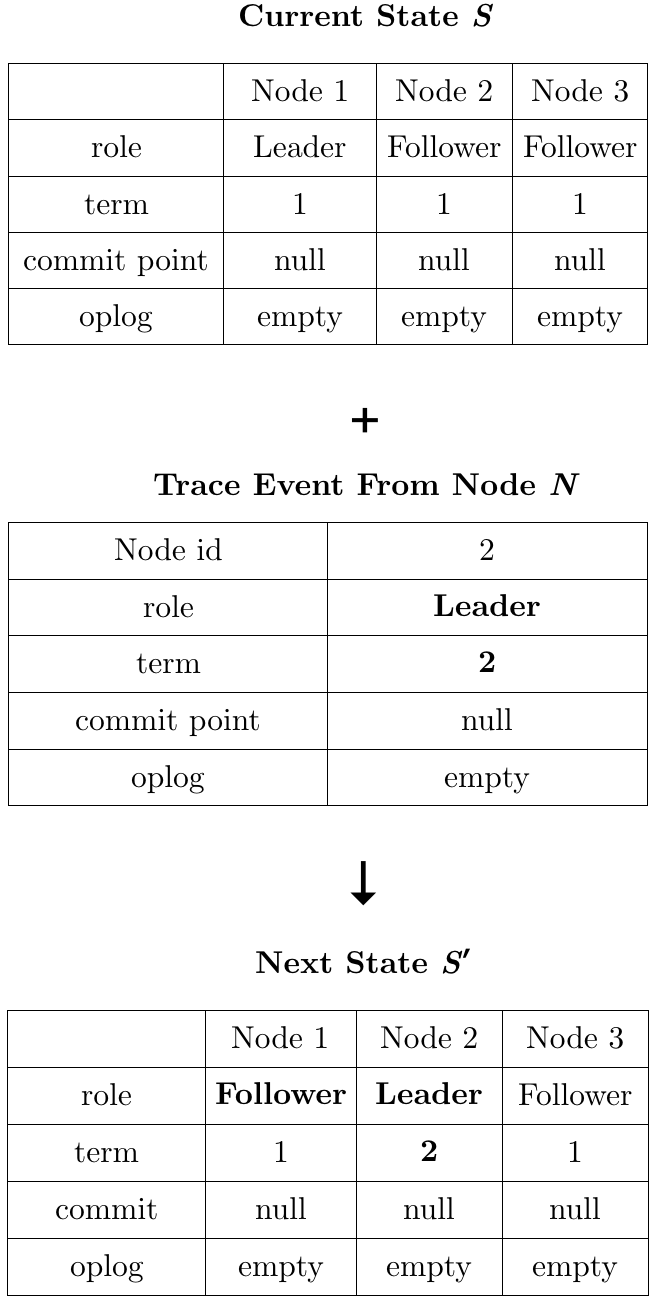
\includegraphics[width=8cm]{event-processing.png}
\caption{Trace Event Processing}
\label{figure:event-processing}
\end{figure}

Once the script constructs this sequence of states, it implements MBTC following a method proposed by Pressler \cite{Pressler18VerifyingSoftwareTracesTLAPlus}: it generates a TLA+ module called \texttt{Trace.tla} which includes the sequence of states (Figure \ref{fig:state-sequence}, a simplification from what our script actually produces), and uses the TLC model-checker to check that the sequence is permitted by the \texttt{RaftMongo.tla} model. The entire data pipeline can be seen in Figure \ref{figure:MBTC-pipline}.

\begin{figure}
\begin{verbatim}
------- MODULE Trace ------------
EXTENDS Integers, Sequences

\* Trace generated from replica set log files. Each
\* tuple is role, term, state, commit point, oplog
\* per node.

Trace == <<
<<
  <<"Leader", "Follower", "Follower">>,
  <<1, 1, 1>>,
  <<NULL, NULL, NULL>>,
  << <<>>, <<>>, <<>> >>
>>,
<<
  <<"Follower", "Leader", "Follower">>,
  <<1, 2, 1>>,
  <<NULL, NULL, NULL>>,
  << <<>>, <<>>, <<>> >>
>>
>>
\end{verbatim}
\caption{State sequence as TLA+ tuple (simplified)}
\label{fig:state-sequence}
\end{figure}

\begin{figure}
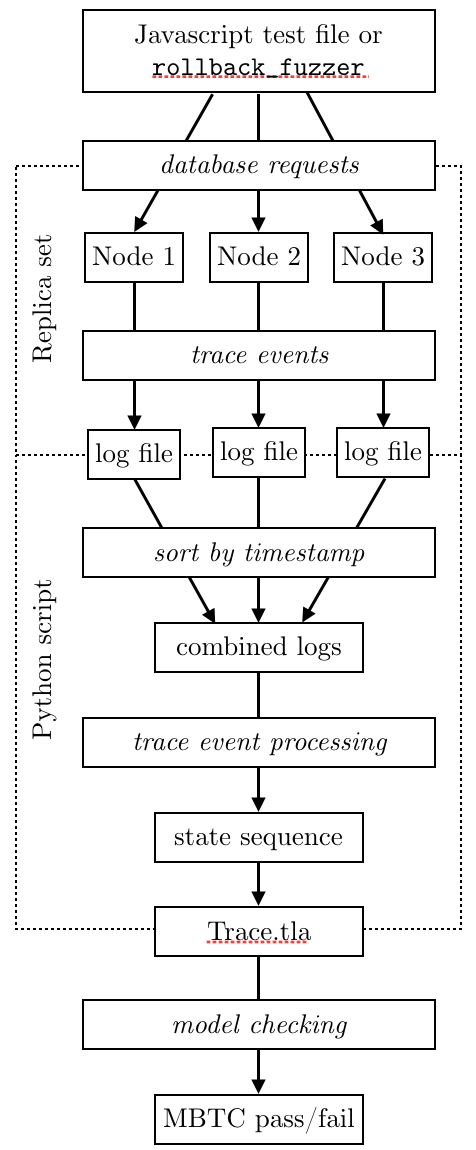
\includegraphics[width=8cm]{MBTC-pipeline.png}
\caption{MBTC data pipeline}
\label{figure:MBTC-pipline}
\end{figure}

\subsection{Analysis}
\label{subsec:mbtc_analysis}

% Probably irrelevant: We considered either a Java harness that fed trace inputs to the TLC internal API, and we tried Pressler's method. Since the former was not fully implemented in Java for us, and the latter already works and includes nice Toolbox diagnostics, we stuck w/ the latter. We also considered Pressler's suggestion of using his method w/ a custom operator that avoids passing through TLA+ tuples as the repr of the trace, we didn't need to do that either.

% Counting from Oct 10, 2019 https://github.com/mongodb-labs/repl-trace-checker/commit/5c96b44d to 
% Jan 10+.
We had intended to trace-check several models against traces from both handwritten and fuzz tests, deploy the trace-checker to our continuous integration system, and measure accumulated state space coverage over all tests. Had we achieved this, we would have built much of the test infrastructure required for eXtreme Modelling.
However, we applied trace-checking to only 5 handwritten tests and one fuzz test, \texttt{rollback\_fuzzer}. 
Only one handwritten test generated traces that passed the trace-checker. 
We did not deploy to continuous integration nor measure coverage. 
The effort to implement MBTC proved so costly for us that we abandoned the project after two and a half months of engineering effort. 
We faced discrepancies between our models and implementation, complexities with concurrency and locking, and incomplete support in TLC. 
In the following sections we describe these issues and propose future solutions.

\subsubsection{Implementation discrepancies}
\label{subsubsec:mbtc_impl_discrepencies}

The first discrepancy we found involved MongoDB's concept of "arbiters".
MongoDB replicas can be configured as arbiters which vote in elections but have no data. 
\texttt{RaftMongo.tla} does not model arbiters and we did not implement tracing for them, thus tests which use arbiters failed when tracing was enabled.
This was trivial to understand and to ignore, but gave us a hint that our specs did not conform to our implementation in as many cases as we wanted---all of them.

Trace checking the output of \texttt{rollback\_fuzzer} immediately reproduced a known violation \cite{SERVER-17934} of the specification: our implementation permits a new follower to acknowledge oplog entries as it syncs them, before it is fully synced with the leader.
This behavior should not be permitted, because it leads to entries being considered majority-committed while part of the majority is still performing an initial sync.
We excluded this behavior from \texttt{RaftMongo.tla} when we first wrote it:
we did not have MBTC in mind, so we deliberately wrote an idealized model, with the intention to eventually bring our implementation into conformance.
When MBTC caught this violation it increased our confidence in trace-checking; however, it was not an acceptable outcome. 
Since the violation came only 4 steps from the trace's start, and the checker stopped at the first violation, the remainder of the 2,683 steps were unchecked. 

To permit \texttt{rollback\_fuzzer} to pass trace-checking, we could 1) fix the implementation sooner than planned, 2) avoid triggering the non-conforming behavior in testing, 3) update the model to match today's implementation, or 4) post-process the traces to simulate a conformant implementation.
Since this particular violation has minimum impact on users, we declined to fix it right away.
Instead we chose solution 2, and modified \texttt{rollback\_fuzzer} to ensure all followers were fully synced before the test began any writes. 

Other discrepancies required solution 3, updating the model. 
For example, \texttt{RaftMongo.tla} originally modeled the election term as a single global number known by all replicas.
This simplification was reasonable when the model was first written, since the election term was not the model's original focus. 
But in fact new election terms are gossiped among replicas, which each learn the new term at a different time.
MBTC required us to make the model more complex to match reality. 
We chose to update the model to resolve this and many other discrepancies: over the course of our research we added or changed 252 of the 345 lines of TLA+ in \texttt{RaftMongo.tla}, costing 3 weeks of effort.

In several cases we chose solution 4, post-processing the logs to simulate conformance. For example, in \texttt{RaftMongo.tla}, when a node joins a replica set it copies the leader's entire oplog.
In the implementation, a new node copies only recent entries.
The \texttt{RaftMongo.tla} behavior more closely matches the Raft protocol that inspired it, and makes it simpler to express invariants such as "an entry is committed after it is replicated to a majority of nodes' oplogs".
Making the implementation conform would discard a useful optimization, and updating the model would have required substantial effort.
Instead we resolved the discrepancy by adding logic to our Python script that filled in the missing entries while it generated the state sequence.
However, such an intrusive modification concerned us: a mistake in the Python script might mask a harmful transcription error in MongoDB.
Given more time, we would have chosen solution 3, and updated the model to match the implementation.

Each discrepancy we discovered through MBTC required us to judge which of the four solutions was cost-effective and would undermine our confidence in the test least. 
Ideally, when an organization practices eXtreme Modelling, they resolve each MBTC failure either by fixing the implementation or, if the failure is not a bug, by updating the model.
In practice, we often judged it was better to work around violations instead of fixing them.
Such workarounds might not have been necessary if we began with a less abstract and idealized model, written for the purpose of MBTC.

\subsubsection{Hierarchical locking, visibility}
\label{subsubsec:mbtc_locking}

Formal specifications of distributed systems algorithms, such as Raft, model a concurrent system of interacting processes, but they typically model each process as single-threaded. 
Production database systems such as MongoDB, however, almost always have high intra-process concurrency and employ some degree of hierarchical locking \cite{Gray76SharedLocks}. 
MongoDB specifically combines a traditional lock manager, with storage-engine Multi-Version Concurrency Control (MVCC), C++ latches, and higher level concurrency control primitives like futures.
It may not be feasible to log a consistent snapshot of such a process's state at the moment of a trace event.

% _tlaPlusRaftMongoEvent_inlock's caller has replcoord mutex, the fn gets Global IS,
% DB IS, and Collection IS locks for local.oplog.rs.
% more details in https://mongodbcr.appspot.com/536420002/, particularly patch set 9
% map locks A, B, C to RSTL, Global, replcoord mutex.

To implement MBTC for \texttt{RaftMongo.tla}, a replica must include the contents of its oplog with each trace event,
but acquiring the locks to obtain a snapshot of the oplog proved difficult. 
Suppose our \texttt{traceLogEvent} procedure (Figure \ref{fig:traceLogEvent}) must acquire locks A, B, and C, in that order, to read the oplog.
Consider a procedure \texttt{becomeLeader} that acquires locks A and C, then changes the replica's role to Leader. 
If we add a call from \texttt{becomeLeader} to \texttt{traceLogEvent}, the latter must acquire lock B, but this is the wrong order and risks deadlocking with other threads.
General solutions are unpalatable: callers of \texttt{traceLogEvent} could be responsible for acquiring all the locks it will need, but this encodes intimate knowledge about \texttt{traceLogEvent} into its callers, and it significantly alters the system's behavior under test.

\begin{figure}
\begin{verbatim}
PROCEDURE becomeLeader() {
    acquire Lock A
    acquire Lock C
    role := Leader
    logTraceEvent()
}

PROCEDURE traceLogEvent() {
    /* Wrong acquisition order if called by
       becomeLeader, risks deadlock */
    acquire Lock A if not yet acquired
    acquire Lock B if not yet acquired
    acquire Lock C if not yet acquired
    read oplog
}
\end{verbatim}
\caption{Pseudocode for a replica becoming a Leader}
\label{fig:traceLogEvent}
\end{figure}

A related challenge was to log each trace event after it had occurred, but \textit{before} the change was visible to other replicas. 
E.g., when a leader receives a write from a client application and creates an oplog entry, it must log the "ClientWrite" event after the entry has appeared in its own oplog, but before any followers can replicate the entry and log an "AppendOplog" event for it. 
If a follower logged an "AppendOplog" event with an earlier timestamp than the leader's "ClientWrite" event, the trace would violate the causal relationship described in the model. 
We had to consider carefully when to log each trace event to achieve this fragile causality.

Solving the two challenges above, for each of the seven named state transitions in \texttt{RaftMongo.tla}, was the single most difficult aspect of our MBTC implementation, costing roughly a month of engineering effort. 
We discovered code locations that obeyed our visibility requirements, and we managed to avoid the need for acquiring locks out of order by exploiting MongoDB's MVCC features: it is possible with our storage engine to read from a snapshot of the oplog, instead of locking the oplog to read its most current contents.
Depending on which state transition was being traced, either reading from a snapshot was correct or locking the oplog was correct and did not risk deadlock.
Fortunately we discovered no cases where neither technique sufficed.
We expect any MBTC implementation for a concurrent database would encounter similar complexities with hierarchical locking and visibility of state changes.

% TODO: oplog truncation had to be papered over in post-processor

We tried to implement MBTC with models written for the sake of documenting and model-checking a design, but we learned that in order to use a formal model with MBTC, the model should be written with MBTC in mind. 
If we began again, we would match our models to the known flaws in the implementation, and faithfully model multi-step events with multiple TLA+ actions.
We would rewrite our specification to model events, such as protocol messages, akin to the original Raft TLA+ model, that are easily observed in the implementation. 
We would try to avoid modelling state that is difficult to snapshot, especially if it were protected with complex locking.
If some state in the model cannot be logged by the implementation, Pressler proposes a "refinement mapping" technique \cite{Pressler18VerifyingSoftwareTracesTLAPlus} that is worth further investigation.

\subsubsection{TLA+ and TLC}
\label{subsubsec:mbtc_tla_tlc}

Tool support for MBTC with TLA+ and TLC is a work in progress. 
Pressler's method worked well to check traces of hundreds of events, but for thousands of events it was impractically slow. 
Pressler proposed, and Markus Alexander Kuppe has begun to implement, features to check long traces by bypassing the TLA+ parser in favor of a special-purpose Java extension to TLC \cite{TLAPlusIssue413}. 
MBTC with TLA+ will be more convenient once these features are finalized and released, with several examples. 
Another missing feature is the ability to combine state-space coverage reports over multiple TLC executions, which would permit engineers to calculate the total coverage achieved by deploying MBTC to continuous integration.

% Debug failures with TLC output or exploration in TLA+ Toolbox GUI

% Estimates of effort, lines of code, MBTC runtime, other statistics


% It's nice to have spec and impl in one repo, and to add spec-specific tracing in the same commits as the spec & impl


% what does MBTC prove?
% Advantage of MBTC over other tests is that implementation tests can't prove liveness, unless you run them forever. TLA+ specs can be checked for liveness, and if the impl matches the spec, the impl might also not have liveness bugs.

% impl is a subset of the spec => if the spec is safe, the impl is safe
% but we can't test to the point where we know that impl is a subset of the spec
% we only know that tested behavior is a subset of the spec

% FALSE: impl is a subset of the spec => if the spec has no liveness bugs, the impl has no liveness bugs
% the impl might lack spec behaviors that are required for liveness

% use "refinement" jargon!

% Reconstruction of truncated oplogs

% Python performance was a bit challenging

% Choices about when to fix conformance in spec, MongoDB, or Python script

% Fixing spec can make it more complex and take longer to model-check and to read
% Might make some configs intractable to model-check that would've been tractable while the spec was more abstract

% the MBTC paper made it sound like adding tracing was easy: they use AspectJ and other Java-specific tech to add fairly non-intrusive logging, with introspection to avoid writing a ton of code, and they don't discuss concurrency problems with getting a point-in-time snapshot of a single process's state. In our highly concurrent C++ application, which is very large and old and not written with MBTC in mind, we found tracing to be the hardest(?) part to implement

% ********************************************************************
% ****************** MBT *********************************************
% ********************************************************************
\section{Model-Based Testing}
\label{sec:model_based_testing}
TODO (Max)
\subsection{Solution}
\label{subsec:mbt_solution}
TODO (Max)
\subsection{Analysis}
\label{subsec:mbt_analysis}
TODO (Max)

% ********************************************************************
% ****************** Conclusions *************************************
% ********************************************************************
\section{Conclusions}
\label{sec:conclusions}

And future work.

% TODO: table layout, fit columns to content

\begin{center}
\begin{tabular}{ | m{11em} | m{5em}| m{6em} | } 
\hline
Task & Effort & Lines of Code \\  
\hline
Event tracing & 4 weeks & 570 C++ \\ 
Update RaftMongo.tla & 3 weeks & 252 TLA+\\ 
Python post-processor & 3 weeks & 484 Python \\ 
\textbf{Total} & \textbf{10 weeks} & \\
\hline
\end{tabular}
\end{center}

%\end{document}  % This is where a 'short' article might terminate

% ensure same length columns on last page (might need two sub-sequent latex runs)
\balance
% ********************************************************************
% ****************** Acknowledgements ********************************
% ********************************************************************
%ACKNOWLEDGMENTS are optional
\section{Acknowledgments}
\label{sec:acknowledgments}
Many experts have advised us, proposed workarounds for obstacles, reviewed our code, and reviewed drafts of this paper, including 
David Bradford,
Mark Callaghan,
Siyuan Zhou,
Will Schultz,
Michael Cahill,
Tess Avitabile,
Henrik Edin,
Andy Schwerin,
and Ron Pressler.
We are embarrassingly indebted to Markus Alexander Kuppe for answering our questions about TLC within minutes, and implementing features we requested within hours.

% The following two commands are all you need in the
% initial runs of your .tex file to
% produce the bibliography for the citations in your paper.
\bibliographystyle{abbrv-original-case}
\bibliography{main}  % use main.bib file
% You must have a proper ".bib" file
%  and remember to run:
% latex bibtex latex latex
% to resolve all references
\end{document}
\balance
